\chapter{Greenhouse Software}
\label{chap:appendix_AllUser}


\section{Login}
\label{sec:appendix_SignIn}
\begin{figure}
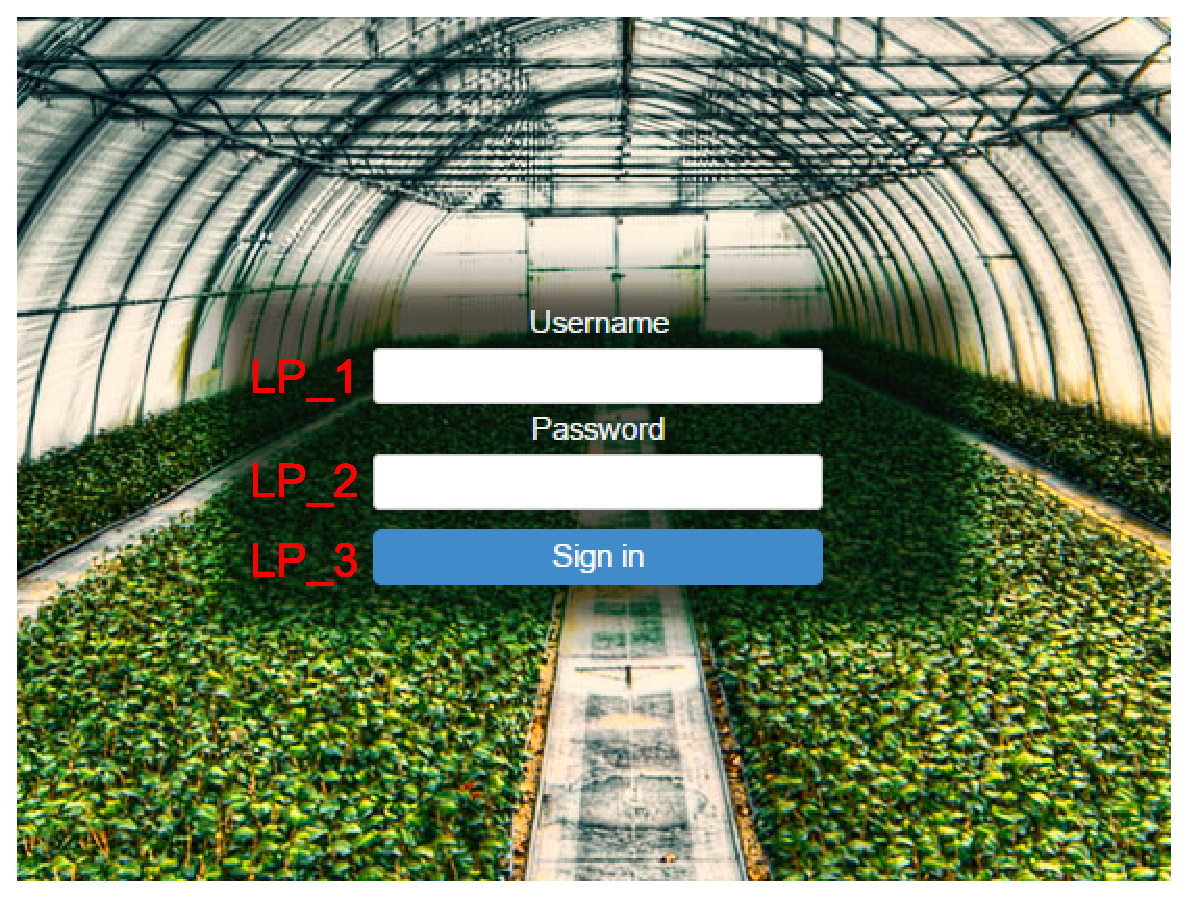
\includegraphics[width=1\textwidth]{images/appendix_images/SignIn.eps}
\end{figure}

The 'Login' page is the first page everyone sees before being able to use any
features of our software.

The User needs to identify himself with valid credentials.
 
\subsection{Username (LP 1)}
This input field is used for the \emph{Username} of the Gardener, Technician or
Manager.

\subsection{Password (LP 2)}
This input field is used for the \emph{Password} of the Gardener, Technician, or
Manager.

\subsection{Sign In Button (LP 3)}
This button send the request to be signed in, by clicking it.

\subsubsection{Success Scenario}
The \emph{User} is taken the \emph{Home} screen.

\subsubsection{Failure Scenario}
The \emph{User} gets a visible error message.


\section{Login}
\label{sec:appendix_SignIn}
\begin{figure}
\includegraphics[width=1\textwidth]{images/appendix_images/GardenRoomRRR.eps}
\end{figure}

The 'Garden'page/screen is the page where all the human actors can look up the
diffrent temperature or light intensity and humidity values in the diffrent
rooms and outside. In addition the screen shows also the actions done by the
system like opening windows or heating,turning on leds and watering the plants
are represented in image format for the given actor.

The given actor needs to be logged in to see this screen.
 
\subsection{Sensor values displayed for room 1 (GR 1)}
The diffrent sensors in room 1 like temperature, light and humidity sensor are
displaying their values inside this given table.

\subsection{Sensor values displayed for room 2 (GR 2)}
The diffrent sensors in room 2 like temperature, light and humidity sensor are
displaying their values inside this given table.

\subsection{Sensor values displayed for room 3 (GR 3)}
The diffrent sensors in room 3 like temperature, light and humidity sensor are
displaying their values inside this given table.

\subsection{Sensor values displayed for room 4 (GR 4)}
The diffrent sensors in room 4 like temperature, light and humidity sensor are
displaying their values inside this given table.

\subsection{Sensor values displayed from outside (GR 5)}
The diffrent sensors from outside like temperature, light and humidity sensor
are displaying their values inside this given table.

\subsection{Sensor values displayed from outside (GR 6)}
These 4 squares displays the 4 rooms. In addition the color of these squeres can
change blue for opening the windows,red for heating a given room. Furthermore
the borders of the square can also change yellow stands for leds turned on and
black of. In addition the watering of plants are displayed by a blue line
connected to the room from the water tank.



\newpage
\section{Home}
\label{sec:appendix_Home}
\mbox{} \par
\noindent\centerimg[width=1\paperwidth]{images/appendix_images/Home.eps}

The \emph{Home} page is the first page the \emph{User} sees after signing in.

This page gives a quick summary of the most important information about the most
recent alerts and warning, the next upcoming tasks and planned watering for each
room and low running stock. 

Further accesses through the blue and white buttons.

\subsection{Schedule (HO 1)}
The \emph{Schedule} shows a summary of the 6 next upcoming tasks of the
gardeners. The list contains information about the \emph{Date}, the \emph{Task
name}, the concerned \emph{Room} and \emph{Gardener} and a checkbox indicating
whether the task is \emph{Important}.

\subsection{Alerts and Warnings (HO 2)}
The \emph{Alerts and Warnings} list shows a summary of the 6 latest Alerts and
Warnings for the \emph{Technician}. The list contains information about the
\emph{Date} and \emph{Time} the alert or warning was added to the system, the
concerned \emph{Room} and \emph{Sensor} if there is a sensor assigned to the
alert or warning. The \emph{Error Type} gives more precise information about the
malfunctioning if it an alert. For Warnings is describes the Problem.
Additionally we get Information about the assigned \emph{Technician} if assigned
and if the problem is already \emph{Solved}.

\subsection{Storage (HO 3)}
The \emph{Storage} list shows a summary of the 6 items with the lowest quantity.
The list contains information about the \emph{Name} of the items, the current
\emph{Amount}. The other information about the \emph{pH-Amount, Vegetable and
TemperaturePref} are used to distinguish between more types of the same plant.

\subsection{Projections (HO 4)}
The \emph{Projections} grid shows a summary of the 4 next rooms planned
to be watered. The single grid contains informations about the concerned
\emph{Room} and the \emph{Date} for the next planned watering.

\subsection{View entire Schedule Button (HO 5)}
The \emph{View entire Schedule} button is a shortcut from the menu
\emph{Schedule} button. The button is designed for a fast access and has a blue
color.

\subsection{View all Alerst and Warnings Button (HO 6)}
The \emph{View all Alerts and Warnings} button is a shortcut from the menu
\emph{Alerts and Projections} button. The button is designed for a fast access
and has a blue color.

\subsection{Manage Storage Button (HO 7)}
The \emph{Manage Storage} button is a shortcut from the menu
\emph{Manager} button. The button is designed for a fast access and has a blue
color.

\subsection{View all Projections Button (HO 8)}
The \emph{View all Projections} button is a shortcut from the menu
\emph{Alerts and Projections} button. The button is designed for a fast access
and has a blue color.

\subsection{Settings Button (HO 9)}
The \emph{Settings} button opens a pop-up window with the \emph{Settings}
screen.

\subsection{View Security Camera Button (HO 10)}
The \emph{View Security Camera} button opens a pop-up window with the
\emph{Security Camera} screen.

\subsection{Exit Button (HO 11)}
The \emph{Exit} button signs the current \emph{User} out and closes the
\emph{Greenhouse} Software application.


\newpage
\section{Statistics}
\label{sec:appendix_Statistics}
\mbox{} \par
\noindent\centerimg[width=\paperwidth]{images/appendix_images/Statistics.eps}

The 'Statistics' page is the  page you see when you navigate to the Statistics
inside the menu. This page helps the operator to see more details and identify
possible problems.

\subsection{Temperature diagram (ST 1)}
The diagram represents the temperature over the last 10 days from the selected
room \textbf{(ST 1.1)}

\subsection{Water Consumption vs Luminosity Level diagram (ST 2)}
The diagram represents the water consumption with the spectral power over 
the last 10 days from the selected room \textbf{(ST 2.1)}

\subsection{Crops statistics (ST 3)}
The crops statistics help the user compare different crops that were harvested and entered into the system.
The compare checkbox \textbf{(ST 3.2)} allows the \emph{User} to select the
panel inside which the crops is loaded.

\subsubsection{Manage button (ST 3.1)}
The 'Manage' button open the Manage crops statistics. This page is only accessible as a \emph{Manager}.


\subsection{Current Stock (ST 4)}
The bar diagram represents the current available stock on seeds.





\newpage
\section{Alerts and Projections}
\label{sec:appendix_AlertsPrejections}
\mbox{} \par
\noindent\centerimg[width=\paperwidth]{images/appendix_images/AlertsProjections.eps}

The 'Alerts and Projections' page is the  page you see when you navigate to the
Alerts and Projections inside the menu. This page helps you to see the current
state of your garden.

\subsection{Alerts Database (AP 1)}
The shown table represents all the lastest alerts and warnings created by the
system. By clicking on the solved checkbox you can mark a warning as solved.

\subsection{Next Watering (AP 2)}
The shown table represents the date of the next watering for each room inside
the database of your system.

\subsection{Next Harvest (AP 3)}
The shown table represents the date of the next harvest for each room inside
the database of your system. These dates are guidelines and your plants may need
more days to be ripe.

\subsection{Water Tank (AP 3)}
The shown table represents the date of the day the water tanks should be
refilled to prevent running dry.





